\chapter{Análisis de requisitos}
\label{chap:use-case}

\section{Introducción}
\label{sec:introduction}

El siguiente diagrama UML representa un resumen visual de los casos de uso que se describirán a continuación: 

\begin{figure}[h]
	\centering
	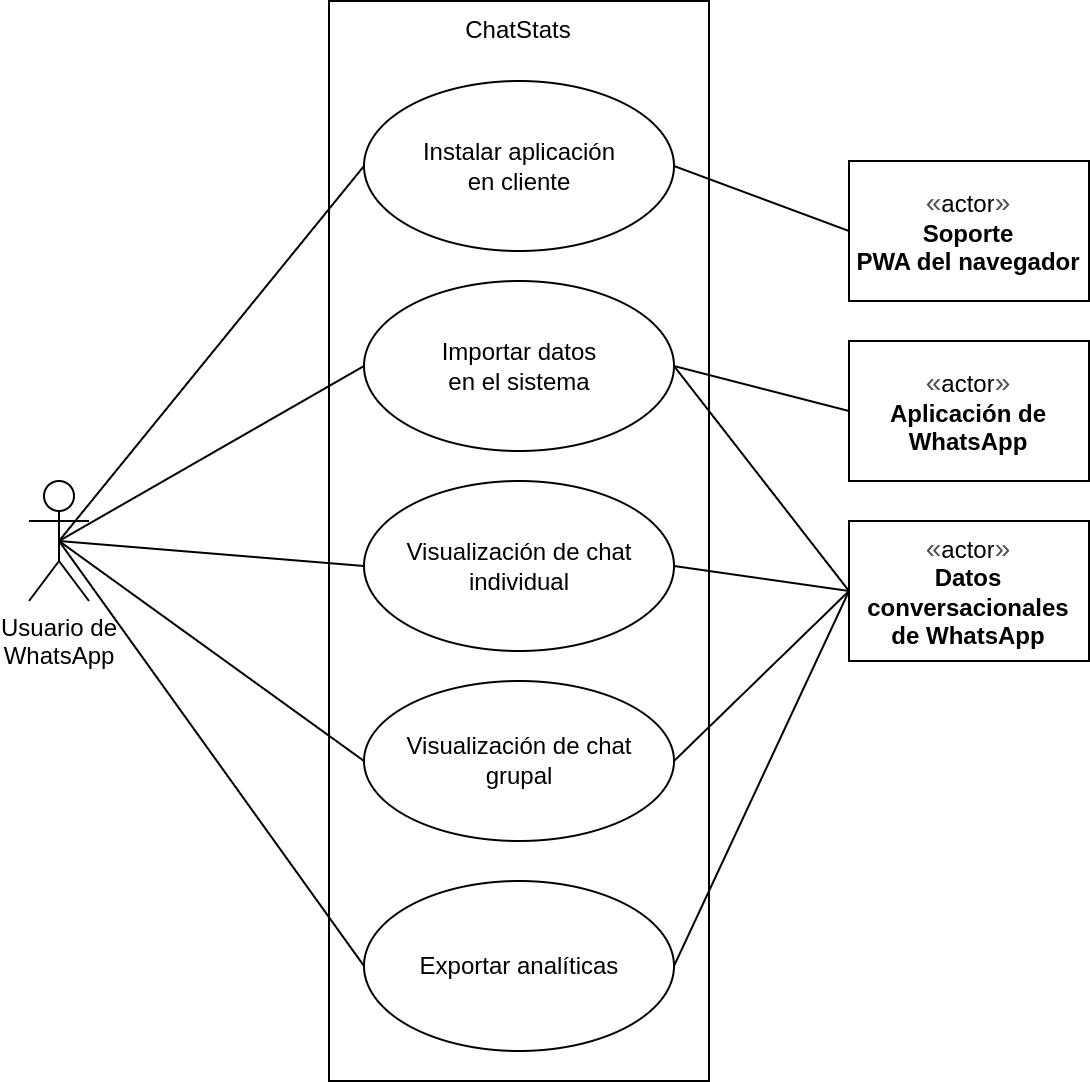
\includegraphics[width=\textwidth]{img/uml.png}
	\caption{Diagrama \acrshort{uml}}
	\label{fig:chap3:uml}
\end{figure}

\section{Casos de uso}
\label{sec:use-cases}


\subsection{Consultar estadísticas y visualizaciones de chat individual sin contenido multimedia}

\subsubsection{Nombre del caso de uso} Consultar estadísticas y visualizaciones de chat individual sin contenido multimedia.

\subsubsection{Actores}

Usuario de WhatsApp.
Navegador con soporte \acrfull{pwa}.
Aplicación WhatsApp
Datos conversacionales de WhatsApp.

\subsubsection{Resumen} El usuario de WhatsApp usará un archivo previamente exportado desde la aplicación WhatsApp como archivo de entrada. Podrá hacerlo desde el explorador de archivos del navegador o compartiendo el archivo en formato \textit{txt} desde el menú de compartir de su sistema operativo, si tiene la \acrfull{pwa} instalada. El archivo no incluirá los mensajes multimedia ni su contenido. Una vez el archivo se ha introducido, el usuario puede confirmar la selección y comenzar el análisis del archivo de texto, cálculo de estadísticas y datos para gráficos. Tras el análisis, se mostrarán las diferentes estadísticas y visualizaciones en la ventana del navegador.

\subsubsection{Secuencia de acciones}

\begin{enumerate}
	\item El usuario introduce el archivo de entrada, ya sea mediante la selección desde el explorador de archivos del navegador, como compartiendo el archivo mediante la \acrshort{pwa} si estuviese instalada.
	\item El usuario confirma la selección del archivo de entrada.
	\item Se realiza el \textit{parseo} del texto, se calculan las estadísticas y se preparan las estructuras de datos para la visualización, mientras el usuario espera en una pantalla de carga. Estas operaciones se realizan en el cliente.
	\item Se muestran gráficos interactivos, así como las estadísticas calculadas previamente.
\end{enumerate}

\begin{comment}
	Debería crear un caso de uso para chats individuales y otro para chats grupales?
	Debería diferenciar el caso de uso de PWA y web normal? (Por la integración con el SO)
	El actor es el archivo exportado y no WhatsApp.
	He cancelado el caso de uso de Telegram puesto que solo puede exportarse desde el ordenador y solo para algunos clientes.
\end{comment}

\subsection{Actores del sistema}
\label{subsec:system-actors}

\subsubsection{Usuario de WhatsApp}

Se trata del usuario único en el que se centran nuestros casos de uso. Este es un usuario de WhatsApp, ya que ChatStats es compatible con los archivos de chat exportados por esta aplicación.

\subsubsection{Navegador con soporte \acrfull{pwa}}

Nuestra aplicación web se ejecuta en un navegador, y por tanto, se trata de un actor para nuestro sistema. Además, si el navegador soporta \acrfull{pwa}, la aplicación web puede ser instalada, ofreciendo mayor integración con el sistema operativo.

\subsubsection{Aplicación WhatsApp}

Para exportar y generar los datos conversacionales que ChatStats espera como entrada, es necesario hacer uso de la aplicación de WhatsApp. Desde dicha aplicación, se puede seleccionar si la exportación se debe realizar con archivos multimedia o sin los mismos.

\subsubsection{Datos conversacionales de WhatsApp}

Es el fichero de datos que nustro sistema espera como entrada. En este caso de uso, se trata de un fichero de texto plano con todos los datos conversacionales exportados por la aplicación WhatsApp para un chat individual, sin incluir los archivos multimedia.

\subsection{Especificación suplementaria}
\label{subsect:suplementary-specification}

\subsubsection{Reglas de dominio}

% Qué eran las reglas de dominio? Qué debería poner aquí?


\subsubsection{Requisitos no funcionales}

\begin{itemize}
	\item \textbf{Interfaces:} leer y analizar archivos de texto plano \textit{txt}. 
	
	\item \textbf{Operación:} Interfaz de Usuario para navegador web, smartphone y tablet.
	
	\item \textbf{Seguridad:} Los datos no deben ser enviados a ningún servidor externo sin la autorización previa del usuario. Estos datos, además, no deben ser almacenados de manera temporal o permanente en ningún servidor. Todas las conexiones entre cliente y servidor deben estar cifradas con SSL.
	
	\item \textbf{Portabilidad:} La aplicación podrá ejecutarse en los navegadores: Chrome, Firefox, Edge y Safari; siendo compatible con \acrshort{pwa} en los navegadores que lo soporten.
\end{itemize}

\subsubsection{Restricciones}
De implementación: lenguaje JavaScript tanto para el servidor como para el cliente, y Docker para el despliegue. El código ha de ser libre.

De interfaz: uso de archivos \textit{txt} para importar los chats exportados desde la aplicación WhatsApp. 

Legales: RGPD.










\subsection{Consultar estadísticas y visualizaciones de chat grupal sin contenido multimedia}

\subsubsection{Nombre del caso de uso} Consultar estadísticas y visualizaciones de chat grupal sin contenido multimedia.

\subsubsection{Actores}

Usuario de WhatsApp.
Navegador con soporte \acrfull{pwa}.
Aplicación WhatsApp
Datos conversacionales de WhatsApp.

\subsubsection{Resumen} El usuario de WhatsApp usará un archivo previamente exportado desde la aplicación WhatsApp como archivo de entrada. Podrá hacerlo desde el explorador de archivos del navegador o compartiendo el archivo en formato \textit{txt} desde el menú de compartir de su sistema operativo, si tiene la \acrfull{pwa} instalada. El archivo no incluirá los mensajes multimedia ni su contenido. Una vez el archivo se ha introducido, el usuario puede confirmar la selección y comenzar el análisis del archivo de texto, cálculo de estadísticas y datos para gráficos. Tras el análisis, se mostrarán las diferentes estadísticas y visualizaciones en la ventana del navegador.

\subsubsection{Secuencia de acciones}

\begin{enumerate}
	\item El usuario introduce el archivo de entrada, ya sea mediante la selección desde el explorador de archivos del navegador, como compartiendo el archivo mediante la \acrshort{pwa} si estuviese instalada.
	\item El usuario confirma la selección del archivo de entrada.
	\item Se realiza el \textit{parseo} del texto, se calculan las estadísticas y se preparan las estructuras de datos para la visualización, mientras el usuario espera en una pantalla de carga. Estas operaciones se realizan en el cliente.
	\item Se muestran gráficos interactivos, así como las estadísticas calculadas previamente.
\end{enumerate}

\begin{comment}
	Debería crear un caso de uso para chats individuales y otro para chats grupales?
	Debería diferenciar el caso de uso de PWA y web normal? (Por la integración con el SO)
	El actor es el archivo exportado y no WhatsApp.
	He cancelado el caso de uso de Telegram puesto que solo puede exportarse desde el ordenador y solo para algunos clientes.
\end{comment}

\subsection{Actores del sistema}
\label{subsec:system-actors}

\subsubsection{Usuario de WhatsApp}

Se trata del usuario único en el que se centran nuestros casos de uso. Este es un usuario de WhatsApp, ya que ChatStats es compatible con los archivos de chat exportados por esta aplicación.

\subsubsection{Navegador con soporte \acrfull{pwa}}

Nuestra aplicación web se ejecuta en un navegador, y por tanto, se trata de un actor para nuestro sistema. Además, si el navegador soporta \acrfull{pwa}, la aplicación web puede ser instalada, ofreciendo mayor integración con el sistema operativo.

\subsubsection{Aplicación WhatsApp}

Para exportar y generar los datos conversacionales que ChatStats espera como entrada, es necesario hacer uso de la aplicación de WhatsApp. Desde dicha aplicación, se puede exportal un chat grupal y seleccionar si la exportación se debe realizar con archivos multimedia o sin los mismos.

\subsubsection{Datos conversacionales de WhatsApp}

Es el fichero de datos que nustro sistema espera como entrada. En este caso de uso, se trata de un fichero de texto plano con todos los datos conversacionales exportados por la aplicación WhatsApp para un chat de grupo, sin incluir los archivos multimedia.

\subsection{Especificación suplementaria}
\label{subsect:suplementary-specification}

\subsubsection{Reglas de dominio}

% Qué eran las reglas de dominio? Qué debería poner aquí?


\subsubsection{Requisitos no funcionales}

\begin{itemize}
	\item \textbf{Interfaces:} leer y analizar archivos de texto plano \textit{txt}. 
	
	\item \textbf{Operación:} Interfaz de Usuario para navegador web, smartphone y tablet.
	
	\item \textbf{Seguridad:} Los datos no deben ser enviados a ningún servidor externo sin la autorización previa del usuario. Estos datos, además, no deben ser almacenados de manera temporal o permanente en ningún servidor. Todas las conexiones entre cliente y servidor deben estar cifradas con SSL.
	
	\item \textbf{Portabilidad:} La aplicación podrá ejecutarse en los navegadores: Chrome, Firefox, Edge y Safari; siendo compatible con \acrshort{pwa} en los navegadores que lo soporten.
\end{itemize}

\subsubsection{Restricciones}
De implementación: lenguaje JavaScript tanto para el servidor como para el cliente, y Docker para el despliegue. El código ha de ser libre.

De interfaz: uso de archivos \textit{txt} para importar los chats exportados desde la aplicación WhatsApp. 

Legales: RGPD.













\subsection{Consultar estadísticas y visualizaciones de chat individual con contenido multimedia}

\subsubsection{Nombre del caso de uso} Consultar estadísticas y visualizaciones de chat individual con contenido multimedia.

\subsubsection{Actores}

Usuario de WhatsApp.
Navegador con soporte \acrfull{pwa}.
Aplicación WhatsApp
Datos conversacionales de WhatsApp.

\subsubsection{Resumen} El usuario de WhatsApp usará un archivo previamente exportado desde la aplicación WhatsApp como archivo de entrada. Podrá hacerlo desde el explorador de archivos del navegador o compartiendo el archivo en formato \textit{txt} desde el menú de compartir de su sistema operativo, si tiene la \acrfull{pwa} instalada. El archivo incluirá los mensajes multimedia. Una vez el archivo se ha introducido, el usuario puede confirmar la selección y comenzar el análisis del archivo de texto, cálculo de estadísticas y datos para gráficos. Tras el análisis, se mostrarán las diferentes estadísticas y visualizaciones en la ventana del navegador, con las visualizaciones de contenido multimedia correspondientes.

\subsubsection{Secuencia de acciones}

\begin{enumerate}
	\item El usuario introduce el archivo de entrada, ya sea mediante la selección desde el explorador de archivos del navegador, como compartiendo el archivo mediante la \acrshort{pwa} si estuviese instalada.
	\item El usuario confirma la selección del archivo de entrada.
	\item Se realiza el \textit{parseo} del texto, se calculan las estadísticas y se preparan las estructuras de datos para la visualización, mientras el usuario espera en una pantalla de carga. Estas operaciones se realizan en el cliente.
	\item Se muestran gráficos interactivos, así como las estadísticas calculadas previamente.
\end{enumerate}

\begin{comment}
	Debería crear un caso de uso para chats individuales y otro para chats grupales?
	Debería diferenciar el caso de uso de PWA y web normal? (Por la integración con el SO)
	El actor es el archivo exportado y no WhatsApp.
	He cancelado el caso de uso de Telegram puesto que solo puede exportarse desde el ordenador y solo para algunos clientes.
\end{comment}

\subsection{Actores del sistema}
\label{subsec:system-actors}

\subsubsection{Usuario de WhatsApp}

Se trata del usuario único en el que se centran nuestros casos de uso. Este es un usuario de WhatsApp, ya que ChatStats es compatible con los archivos de chat exportados por esta aplicación.

\subsubsection{Navegador con soporte \acrfull{pwa}}

Nuestra aplicación web se ejecuta en un navegador, y por tanto, se trata de un actor para nuestro sistema. Además, si el navegador soporta \acrfull{pwa}, la aplicación web puede ser instalada, ofreciendo mayor integración con el sistema operativo.

\subsubsection{Aplicación WhatsApp}

Para exportar y generar los datos conversacionales que ChatStats espera como entrada, es necesario hacer uso de la aplicación de WhatsApp. Desde dicha aplicación, se puede seleccionar si la exportación se debe realizar con archivos multimedia o sin los mismos. Este caso de uso comprende la exportación con contenido multimedia.

\subsubsection{Datos conversacionales de WhatsApp}

Es el fichero de datos que nustro sistema espera como entrada. En este caso de uso, se trata de un fichero de texto plano con todos los datos conversacionales exportados por la aplicación WhatsApp para un chat individual, incluyendo los archivos multimedia.

\subsection{Especificación suplementaria}
\label{subsect:suplementary-specification}

\subsubsection{Reglas de dominio}

% Qué eran las reglas de dominio? Qué debería poner aquí?


\subsubsection{Requisitos no funcionales}

\begin{itemize}
	\item \textbf{Interfaces:} leer y analizar archivos de texto plano \textit{txt}. 
	
	\item \textbf{Operación:} Interfaz de Usuario para navegador web, smartphone y tablet.
	
	\item \textbf{Seguridad:} Los datos no deben ser enviados a ningún servidor externo sin la autorización previa del usuario. Estos datos, además, no deben ser almacenados de manera temporal o permanente en ningún servidor. Todas las conexiones entre cliente y servidor deben estar cifradas con SSL.
	
	\item \textbf{Portabilidad:} La aplicación podrá ejecutarse en los navegadores: Chrome, Firefox, Edge y Safari; siendo compatible con \acrshort{pwa} en los navegadores que lo soporten.
\end{itemize}

\subsubsection{Restricciones}
De implementación: lenguaje JavaScript tanto para el servidor como para el cliente, y Docker para el despliegue. El código ha de ser libre.

De interfaz: uso de archivos \textit{txt} para importar los chats exportados desde la aplicación WhatsApp. 

Legales: RGPD.







\subsection{Consultar estadísticas y visualizaciones de chat grupal con contenido multimedia}

\subsubsection{Nombre del caso de uso} Consultar estadísticas y visualizaciones de chat grupal con contenido multimedia.

\subsubsection{Actores}

Usuario de WhatsApp.
Navegador con soporte \acrfull{pwa}.
Aplicación WhatsApp
Datos conversacionales de WhatsApp.

\subsubsection{Resumen} El usuario de WhatsApp usará un archivo previamente exportado desde la aplicación WhatsApp como archivo de entrada. Podrá hacerlo desde el explorador de archivos del navegador o compartiendo el archivo en formato \textit{txt} desde el menú de compartir de su sistema operativo, si tiene la \acrfull{pwa} instalada. El archivo incluirá los mensajes multimedia del grupo. Una vez el archivo se ha introducido, el usuario puede confirmar la selección y comenzar el análisis del archivo de texto, cálculo de estadísticas y datos para gráficos. Tras el análisis, se mostrarán las diferentes estadísticas y visualizaciones en la ventana del navegador, con las visualizaciones de contenido multimedia correspondientes.

\subsubsection{Secuencia de acciones}

\begin{enumerate}
	\item El usuario introduce el archivo de entrada, ya sea mediante la selección desde el explorador de archivos del navegador, como compartiendo el archivo mediante la \acrshort{pwa} si estuviese instalada.
	\item El usuario confirma la selección del archivo de entrada.
	\item Se realiza el \textit{parseo} del texto, se calculan las estadísticas y se preparan las estructuras de datos para la visualización, mientras el usuario espera en una pantalla de carga. Estas operaciones se realizan en el cliente.
	\item Se muestran gráficos interactivos, incluyendo las visualizaciones multimedia, así como las estadísticas calculadas previamente.
\end{enumerate}

\subsection{Actores del sistema}
\label{subsec:system-actors}

\subsubsection{Usuario de WhatsApp}

Se trata del usuario único en el que se centran nuestros casos de uso. Este es un usuario de WhatsApp, ya que ChatStats es compatible con los archivos de chat exportados por esta aplicación.

\subsubsection{Navegador con soporte \acrfull{pwa}}

Nuestra aplicación web se ejecuta en un navegador, y por tanto, se trata de un actor para nuestro sistema. Además, si el navegador soporta \acrfull{pwa}, la aplicación web puede ser instalada, ofreciendo mayor integración con el sistema operativo.

\subsubsection{Aplicación WhatsApp}

Para exportar y generar los datos conversacionales que ChatStats espera como entrada, es necesario hacer uso de la aplicación de WhatsApp. Desde dicha aplicación, se puede seleccionar si la exportación se debe realizar con archivos multimedia o sin los mismos. Este caso de uso comprende la exportación con contenido multimedia.

\subsubsection{Datos conversacionales de WhatsApp}

Es el fichero de datos que nustro sistema espera como entrada. En este caso de uso, se trata de un fichero de texto plano con todos los datos conversacionales exportados por la aplicación WhatsApp para un chat grupal, incluyendo los archivos multimedia.

\subsection{Especificación suplementaria}
\label{subsect:suplementary-specification}

\subsubsection{Reglas de dominio}

% Qué eran las reglas de dominio? Qué debería poner aquí?


\subsubsection{Requisitos no funcionales}

\begin{itemize}
	\item \textbf{Interfaces:} leer y analizar archivos de texto plano \textit{txt}. 
	
	\item \textbf{Operación:} Interfaz de Usuario para navegador web, smartphone y tablet.
	
	\item \textbf{Seguridad:} Los datos no deben ser enviados a ningún servidor externo sin la autorización previa del usuario. Estos datos, además, no deben ser almacenados de manera temporal o permanente en ningún servidor. Todas las conexiones entre cliente y servidor deben estar cifradas con SSL.
	
	\item \textbf{Portabilidad:} La aplicación podrá ejecutarse en los navegadores: Chrome, Firefox, Edge y Safari; siendo compatible con \acrshort{pwa} en los navegadores que lo soporten.
\end{itemize}

\subsubsection{Restricciones}
De implementación: lenguaje JavaScript tanto para el servidor como para el cliente, y Docker para el despliegue. El código ha de ser libre.

De interfaz: uso de archivos \textit{txt} para importar los chats exportados desde la aplicación WhatsApp. 

Legales: RGPD.